% =====================================================================
\section{The OELLM Benchmark}
\label{sec:dataset}
% =====================================================================

We build \textbf{OELLM}, a deterministic, OpenStreetMap-grounded benchmark that
pairs overhead and street-level imagery to make the question \emph{``when does a
second view help?''} measurable. Every answer derives from OSM tags or coordinate
geometry rather than human annotation, so the corpus is bit-exact reproducible and
carries no annotator drift. We describe the construction, the task taxonomy, the
splits, and the evaluation protocol, and state the trade-off honestly: the
benchmark is limited to what OSM and geometry can certify, but every answer is
verifiable and the same OSM snapshot regenerates the same questions.

\subsection{Construction}
\label{sec:construction}
Each \emph{location} is sampled within one of \num{40} cities across \num{32}
countries on six continents and is associated with (i) one satellite tile, (ii)
four street-level views at fixed road-aligned bearings (forward, backward, left,
right), and (iii) OSM-derived attribute labels. A seven-stage pipeline
(\cref{fig:pipeline}) threads each sample through location sampling, satellite-tile
fetching, street-view capture, OSM enrichment, composite rendering, deterministic
question generation, and validation/splitting.

\begin{figure}[t]
  \centering
  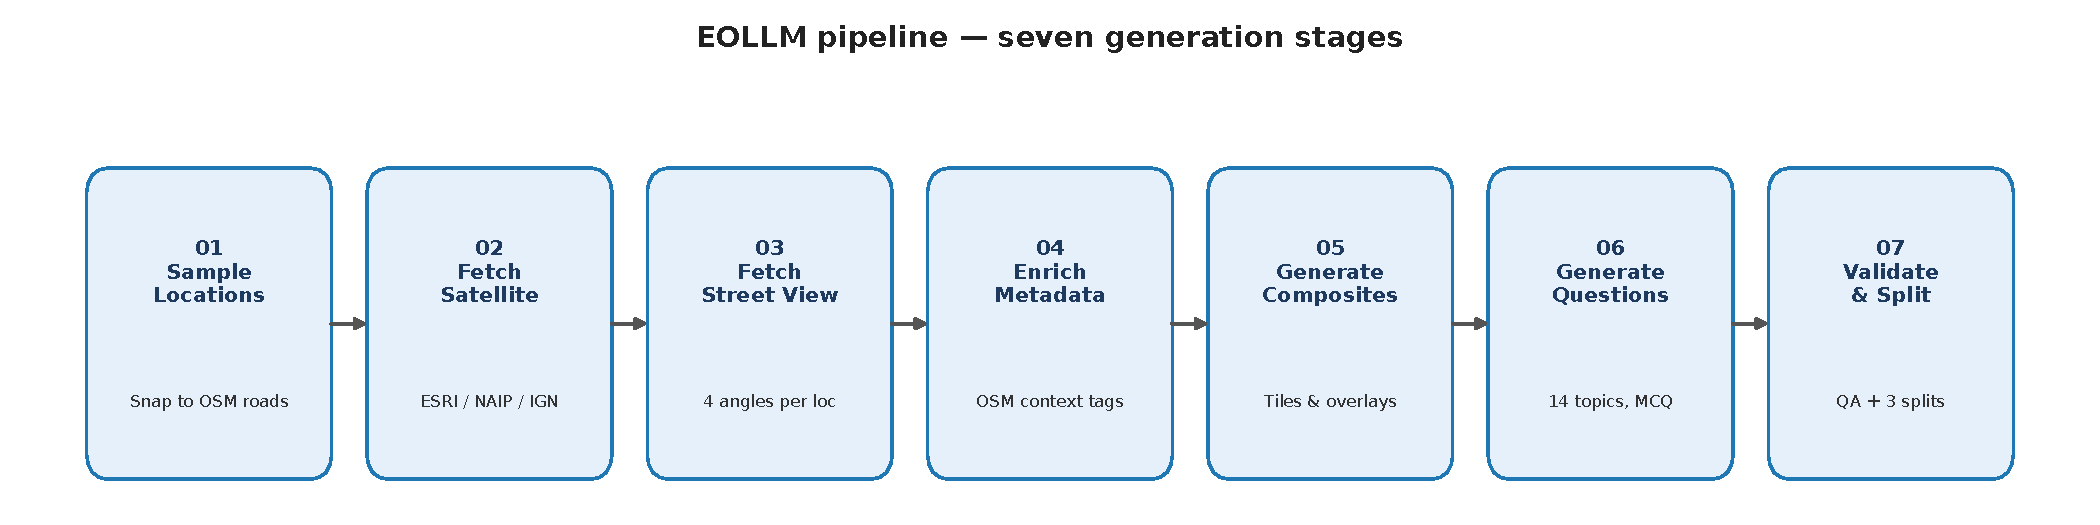
\includegraphics[width=\linewidth]{figures/fig13_pipeline.pdf}
  \caption{The seven-stage deterministic generation pipeline. Every stage reads and
  enriches the same list of sample dictionaries; no human annotation is involved.}
  \label{fig:pipeline}
\end{figure}

Satellite imagery is sourced per location by geography---sub-meter aerial
orthophotos: ESRI World Imagery ($\sim$\SIrange{0.3}{0.5}{m/px} in cities) as the
global default, NAIP ($\sim$\SI{0.6}{m/px}) in the US, and IGN ($\sim$\SI{0.2}{m/px})
in France, with a coarse Sentinel-2 fallback ($\sim$\SI{10}{m/px}) reserved for
locations no high-resolution source covers. Across the \num{34484}-record corpus,
\num{31489} questions (\num{91}\%) draw ESRI imagery, \num{1946} NAIP, and
\num{1049} IGN; the Sentinel-2 fallback was never triggered, so the redundancy we
report later is measured against uniformly sub-meter overhead imagery rather than a
coarse proxy. The satellite tile carries a marker indicating the queried location;
the marker is part of the input and is held fixed across all ablation modes (its
effect is examined in \cref{sec:robustness}). Street-level views are retrieved from
Google Street View and retain Google's original attribution; satellite imagery is
\copyright\ its respective provider (Esri, NAIP/USDA, IGN).

\subsection{Task taxonomy}
\label{sec:taxonomy}
The benchmark contains \num{12} task families in two groups
(\cref{fig:examples}). Two satellite-only tasks present in earlier drafts,
\textsf{green\_space} and \textsf{road\_surface}, were \emph{retired} from the
released benchmark because every model we evaluated solved them almost perfectly
and they therefore carried no discriminative signal; we discuss this audit in
\cref{sec:robustness} and report on the \num{10} retained tasks below.

\paragraph{Urban understanding (seven tasks).}
\textsf{land\_use}, \textsf{building\_height}, \textsf{urban\_density},
\textsf{road\_type}, \textsf{junction\_type}, \textsf{amenity\_richness}, and
\textsf{transit\_density}. Each is a four-way multiple-choice question whose answer
follows from one location's OSM context; the visual is a marked satellite tile plus
street-level imagery. These are the tasks for which ``do we need both views?'' is
well-posed, because each is in principle answerable from imagery of a single
location.

\paragraph{Cross-view geolocalisation (five tasks).}
\textsf{camera\_direction} asks which of four arrows on the satellite tile points
in the heading a single street view was captured from;
\textsf{mismatch\_binary\_\{easy,hard\}} ask whether a street-view set belongs to a
satellite tile; \textsf{mismatch\_mcq\_\{easy,hard\}} ask which of four street-view
composites matches the tile. \emph{Easy} variants draw distractors from another
city (where vegetation, signage language, and vehicle types often leak the answer);
\emph{hard} variants draw them from the same city, defeating those shortcuts and
isolating the geometric match. These answers live in the \emph{relationship}
between views and are unanswerable from a single view by construction.

\paragraph{A fair test of fusion.}
The two groups differ in what fusion can buy, and this difference is the benchmark's
design principle. An urban-attribute question is, by construction, answerable in
principle from \emph{either} modality, and empirically each single view alone
carries the answer: for most urban tasks the satellite-only and street-only
accuracies of our trained model track each other closely (e.g.\ \textsf{land\_use}
\num{72.4} vs.\ \num{71.7}, \textsf{building\_height} \num{60.0} vs.\ \num{62.6},
\textsf{road\_type} \num{72.7} vs.\ \num{76.0}; \cref{sec:main}). The question is
therefore not whether one view \emph{can} suffice but whether a model \emph{gains}
from holding both---a fair test of fusion precisely because each view is
independently sufficient. The cross-view group is the complement: a class of tasks
that genuinely \emph{require} fusion, included so the same instrument can register
large synergy when fusion is the only route to the answer. We do not claim urban
semantics can never require cross-view reasoning; we claim that the attribute tasks
deployed in current urban-VLM benchmarks do not, and we provide the cross-view
group to exhibit tasks that do.

\subsection{Splits}
\label{sec:splits}
All splits operate at the location level, so no location's questions span two
splits. We hold out a disjoint \emph{benchmark} of \num{4734} questions (all
\num{12} released tasks) drawn from a mixture of seen and unseen cities, shipped in
two parallel files (\texttt{public}, no answers; \texttt{with\_answers},
gold-labelled). For training we use two strategies that share this benchmark
(\cref{tab:dataset}): a \emph{per-city} split (random locations per city to
validation) and a \emph{seen/unseen} split (eight cities held out entirely, probing
geographic generalisation). Our primary model is trained on the seen/unseen split.
Question generation seeds option shuffling from \texttt{sample\_id}\,$+$\,topic, so
the correct letter is stable across re-runs but distributed across the corpus; we
keep one question per (location, task) pair to avoid location-level inflation, and
discard locations with fewer than four street-level views.

\begin{table}[t]
  \centering
  \caption{Record counts for the released OELLM corpus (\num{34484} questions over
  \num{4168} locations in \num{40} cities). Two training strategies share one
  disjoint benchmark. This paper's fusion audit uses the seven urban-attribute
  tasks of the benchmark ($n=\num{2629}$); the remaining \num{2105} cross-view
  questions form the positive control of \cref{sec:control}.}
  \label{tab:dataset}
  \setlength{\tabcolsep}{8pt}
  \begin{tabular}{@{}lrrr@{}}
    \toprule
    Split set & Train & Validation & Benchmark \\
    \midrule
    per\_city    & \num{23431} & \num{6319} & --- \\
    seen\_unseen & \num{23282} & \num{8179} & --- \\
    benchmark (12 tasks) & --- & --- & \num{4734} \\
    \bottomrule
  \end{tabular}
\end{table}

\subsection{Evaluation protocol}
\label{sec:protocol}
We evaluate every model under a controlled \emph{image ablation}: each question is
posed under four input conditions---\textsf{blind} (question and options only),
\textsf{sat} (the marked satellite tile only), \textsf{sv} (street-level view only),
and \textsf{full} (both). The text of the question and options is byte-identical
across conditions; only the supplied images change. We decode greedily with a fixed
seed and parse a single answer letter with a strict word-boundary matcher; the same
harness, prompt, and rendering run across all models so that only the forward pass
differs. Of the \num{4734} benchmark questions spanning all \num{12} released tasks,
this study's fusion audit uses the \num{2629} questions from the seven
urban-attribute tasks; the remaining \num{2105} cross-view questions serve as the
positive control. Per-task question counts are uneven by design, reflecting OSM-tag
availability rather than importance (\textsf{building\_height}, \num{190};
\textsf{junction\_type}, \num{334}; the other five urban tasks, \num{421} each).

\subsection{Coverage and limitations}
\label{sec:coverage}
We flag two forms of uneven coverage. Geographically the corpus is Europe-weighted
(the single largest share of records), with the remaining cities spread across five
other continents; absolute accuracies should be read with that skew in mind, though
our headline metric is computed within each question and is unaffected by the
geographic mix. Label-wise, a few attribute tasks depend on OSM tags that are
sparse in some cities---\texttt{building:levels}, which underlies
\textsf{building\_height}, is sparse in São Paulo and Singapore---so those tasks
contribute fewer questions. Full distributional statistics are provided in the
accompanying dataset report.
